% !TEX root = C:\Users\Jan\Documents\dev\Risk-Measurement-Framework\masterthesis_tex\masterthesis_main.tex
\section{Evaluation}
\label{sec:evaluation}

A common example to show backdoor attacks is traffic sign detection (\cite{DBLP:journals/corr/abs-2102-10369}, \cite{DBLP:journals/corr/abs-1708-06733}, \cite{DBLP:conf/codaspy/NudingM20},
\cite{DBLP:journals/tdsc/LiXZZZ21}). That makes it easier to find datasets and already finished ML models to make a case study. In the following subsections the focus lies on the case study which concept and its implementation is evaluated here. \\ Further, the requirements and procedures from ISO 27004 in relation with the RMF is discussed in this section. In addition, this section describes real-world examples for which the RMF could be used.

\subsection{Evaluation of the ISO 27004 standard in context to the RMF}

Sections \ref{sec:conFrame} and \ref{sec:implementation} show both that it is possible to design and implement a technical framework for ML security especially risk measurement based on ISO 27004 \cite{ISO_27004_2009} which answers \ref{itm:rq1}. Also, the decisions that come individually from the organization had to be disregarded by using specific attacks and risk indicators because there is no choice available at this point. However, as soon as individual decisions are required, such as information needs and stakeholder identification, it is no longer possible to implement this without human decisions. In summary, hypothesis \ref{itm:h3} - \textit{It is possible to design and implement a risk measurement framework for ML models based on the generalized requirements of ISO 27004} can be confirmed at this point.

\subsection{Case Study: Developing a SVM for traffic sign detection}

For the case study scikit-learn \cite{scikit-learn} and for preparation of the dataset in Python OpenCV2 have different function to load and resize images \cite{opencv_library}. In their work, Stallkamp et al. \cite{DBLP:conf/ijcnn/StallkampSSI11} built a mulit-category classification dataset. The mulit-category classification dataset contains german traffic signs for image classification. That mulit-category classification dataset uses the german traffic signs from a approx. 10 hours daytime video from different roads.
This case study is an example to show the functions and results of the RMF. After showing this case study there will be explain and discuss realistic case studies where backdoor attacks could have a more realistic impact for scores of ML models.

\subsubsection*{Structure of the ML model for the case study}

The original dataset from Stallkamp et al. \cite{DBLP:conf/ijcnn/StallkampSSI11} is splitted between a training and testing folder. The training folder separate 43 signs into subfolders. This subfolders make it easy to use specific traffic signs which decrease the training time. The information of the folders are written in an eponymous csv-file that are not needed further in this case study. In Figure \ref{fig:traffic_signs} the shown traffic signs can be used for training the SVM and are all labeled in the data preprocessing like the subfolder name 0 - 42. The training set contains traffic signs such as speed limit, prohibitory, derestriction, mandatory, danger, and unique signs.

\begin{figure}[h!]
  \centering
  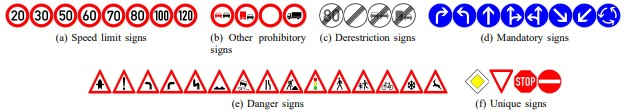
\includegraphics[width=12cm]{pictures/traffic_signs.jpg}
  \caption{Labeled traffic signs adapted from \cite{DBLP:conf/ijcnn/StallkampSSI11}.}
  \label{fig:traffic_signs}
\end{figure}

\begin{figure}[h!]
  \centering
  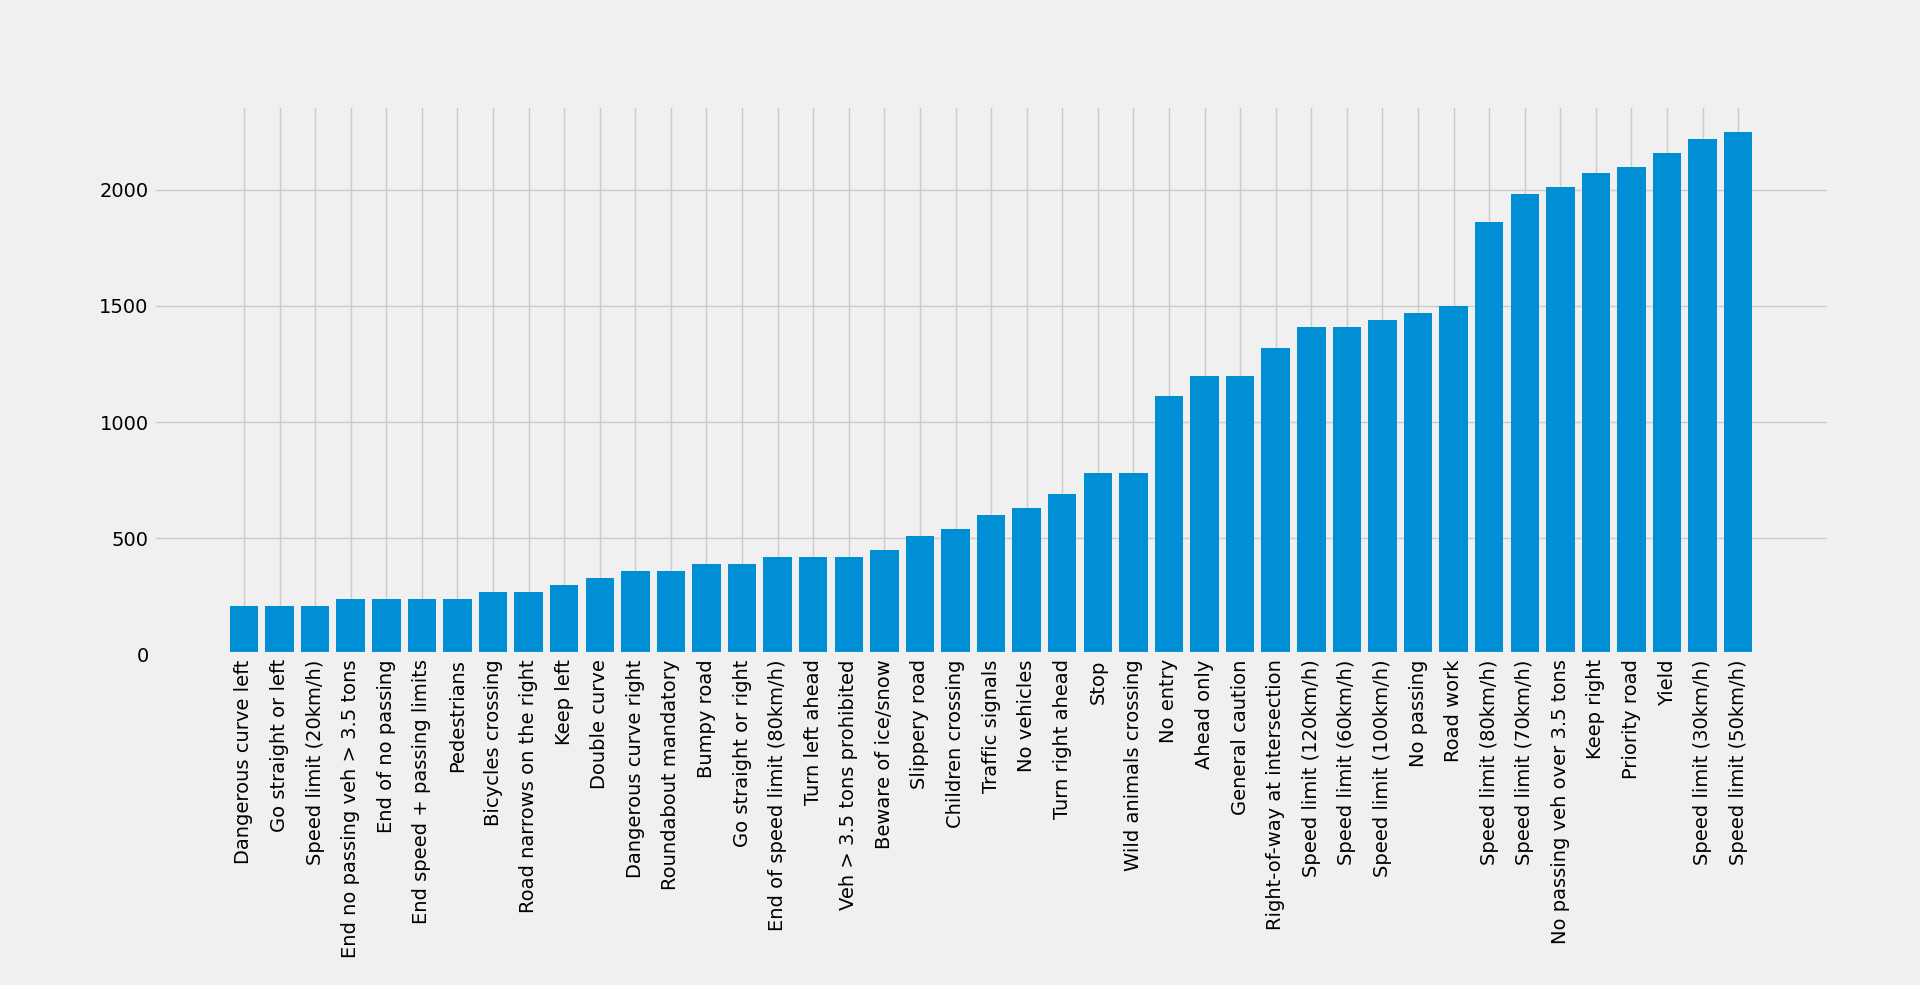
\includegraphics[width=15cm]{pictures/num_of_images.png}
  \caption{Number of images per labels.}
  \label{fig:num_of_images}
\end{figure}

All signs are resized to 50x50 pixel to optimize the performance of the NN. The training sets are also scaled with Keras and TensorFlow to execute the attacks successfully. The training data and test data load from two different folders and are trained during ten epochs. All functions, the arguments and a description of them can be found in appendix \ref{sec:case_study_functions}. Figure \ref{fig:nn} shows the NN architecture.

\begin{figure}[h!]
  \centering
  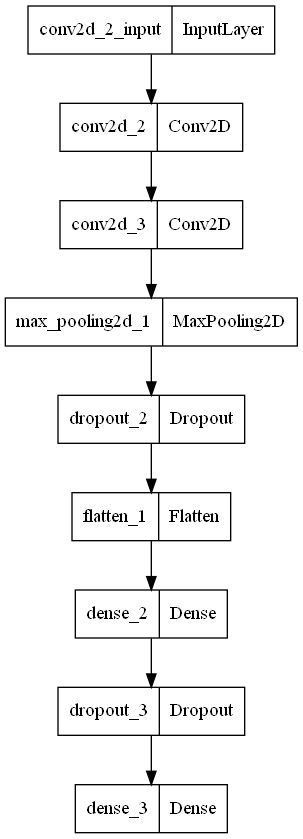
\includegraphics[width=5cm]{pictures/nn.png}
  \caption{Generated NN architecture image from Keras.}
  \label{fig:nn}
\end{figure}

The computer to execute the ML model have resources such as, AMD Ryzen \cite{DBLP:conf/hotchips/AroraBW20} 7 5800X 8-Core Processor with 3.80 GHz, 16 GB of RAM, and a NVIDIA GeForce RTX \cite{DBLP:journals/pcs/SanzharovFG20} 3060 Ti. These resources are available to the attacker and to measure the computational resources to get the attacker's effort.

\subsection{Differences between manipulated and original dataset}

\begin{figure}[ht!]
  \centering
  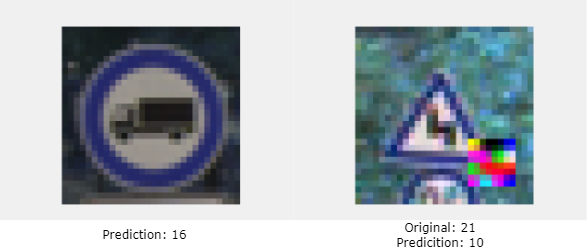
\includegraphics[width=10cm]{pictures/backdoor_example_rmf.png}
  \caption{The left image shows a clean output. The right image shows a poisoned output with a wrong prediction. Both images are the output from the ML model with the \textit{Clean Label Backdoor Attack} from the RMF.}
  \label{fig:backdoor_example_rmf}
\end{figure}

The Python plots from the case study show in this subsection examples images to show the differences between the original and manipulated dataset. Figure \ref{fig:backdoor_example_rmf} visualizes the prediction of the ML model with the attack of the RMF. If the ML model is executed multiple times, the poisoned image show always the same wrong label because the attack specificity is targeted.

\subsection{Results from the measurement methods}

For this case study, the ML model is attacked by a \textit{Clean Label Backdoor Attack} with a backdoor trigger that Figure \ref{fig:poisoned_hidden_trigger} shows. $50\%$ of the images are poisoned during the attack to missclassify to the label \textit{10: No passing veh over 3.5 tons}.

\subsubsection*{Risk indicators to measure the attacker's effort}

\noindent\textbf{Attacker's goal} As the attack is a backdoor attack, the RMF returns for the attacker's goal an inference failure. It takes six steps to develop a backdoor attack. These development steps are generalized and base not on a specific attack. The RMF returned these six steps as a natural number which shows, that the RMF measured the correct goal. \\

\noindent\textbf{Attacker's knowledge} This risk indicator returned the number of steps to implement the \textit{Clean Label Backdoor Attack}. Based on the work of Turner et al. \cite{turner2018clean}, this thesis figured out that it takes ten steps to implement this attack. The ART \cite{art2018} define which information are to be used as parameters to execute this attack. \\

\noindent\textbf{Computational resources} The computational resources that are measured are the CPU, GPU, and RAM. The RAM measurement starts at the beginning of the implemented ML model and shows after finishing the training time of the ML model how much RAM resources the ML model uses. The CPU and GPU are measured directly after the training without a start point. The training time with the implemented attack uses $1825.73MB$ RAM, $9\%$ CPU, and $8137.81MB$ of the GPU. The CPU and RAM measurement do not measure the training time of the ML model, but from the complete Python program. \\ \\

Considering the individual risk indicators, these show the effort. At this point, however, the comparison to values describing a lower or higher effort is missing. While this can answer research question \ref{itm:rq3} - \textit{What are risk indicators to measure the attacker's effort?} that the above risk indicators describe the effort of an attacker as well as the hypothesis \ref{itm:h2} - \textit{There are several risk indicators to measure the attacker's effort when attacking a ML model: \textbf{(a)} computational resources \textbf{(b)} attacker's goal \textbf{(c)} attacker's knowledge} can be confirmed. Nevertheless, the comparative values are missing what is missing of a complete confirmation and answer.

\subsubsection*{Risk indicators to measure the extent of damage}

\noindent\textbf{Attack time} All backdoor attacks are executing during training time. Figure \ref{fig:feature_match} shows that FLANN and SIFT found the backdoor in a poisoned image. The time to train a ML model with the attack and inference time takes $1037.23$ seconds.

\begin{table}[ht!]
\centering
  \begin{tabular}{| l | p{1.5cm} | p{2cm} | p{1.5cm} | p{1.5cm} |}
  \hline
  \rowcolor{lightgray} Label & TP & TN & FP & FN \\ [0.5ex]
  \hline
  Speed limit (20km/h) & 59, 0 & 12570, 11911 & 0, 0 & 1, 59\\
  \hline
  Speed limit (30km/h) & 707, 2 & 11898, 11220 & 12, 66 & 13, 682\\
  \hline
  Speed limit (50km/h) & 743, 5 & 11873, 11217 & 7, 51 & 7, 697\\
  \hline
  Speed limit (60km/h) & 430, 0 & 12169, 11555 & 11, 0 & 20, 415\\
  \hline
  Speed limit (70km/h) & 655, 1 & 11959, 11331 & 11, 2 & 5, 636\\
  \hline
  Speed limit (80km/h) & 620, 0 & 11953, 11377 & 47, 0 & 10, 593\\
  \hline
  End of speed limit (80km/h) & 132, 0 & 12480, 11827 & 0, 0 & 18, 143\\
  \hline
  Speed limit (100km/h) & 428, 0 & 12175, 11541 & 5, 0 & 22, 429\\
  \hline
  Speed limit (120km/h) & 431, 0 & 12173, 11546 & 7, 0 & 19, 424\\
  \hline
  No passing & 479, 0 & 12132, 11519 & 18, 0 & 1, 451\\
  \hline
  No passing veh over 3.5 tons & 656, 560 & 11968, 1242 & 2, 10100 & 4, 68\\
  \hline
  Right-of-way at intersection & 416, 0 & 12204, 11567 & 6, 0 & 4, 403\\
  \hline
  Priority road & 682, 12 & 11937, 11129 & 3, 179 & 8, 650\\
  \hline
  Yield & 718, 0 & 11907, 11273 & 3, 11 & 2, 686\\
  \hline
  Stop & 269, 0 & 12360, 11709 & 0, 0 & 1, 261\\
  \hline
  \end{tabular}
  \caption{True and False values (left) before the attack, (right) after the attack.}
  \label{tab:pos_neg_1}
\end{table}

\begin{table}[ht!]
\centering
  \begin{tabular}{| l | p{1.5cm} | p{2cm} | p{1.5cm} | p{1.5cm} |}
  \hline
  \rowcolor{lightgray} Label & TP & TN & FP & FN \\ [0.5ex]
  \hline
  No vehicles & 210, 0 & 12413, 11772 & 7, 0 & 0, 198\\
  \hline
  Veh > 3.5 tons prohibited & 149, 0 & 12478, 11828 & 2, 0 & 1, 142\\
  \hline
  No entry & 351, 2 & 12269, 11539 & 1, 83 & 9, 346\\
  \hline
  General caution & 383, 1 & 12229, 11581 & 11, 22 & 7, 366\\
  \hline
  Dangerous curve left & 60, 0 & 12562, 11915 & 8, 0 & 0, 55\\
  \hline
  Dangerous curve right & 89, 0 & 12522, 11888 & 18, 0 & 1, 82\\
  \hline
  Double curve & 84, 0 & 12538, 11885 & 2, 0 & 6, 85\\
  \hline
  Bumpy road & 109, 0 & 12509, 11858 & 1, 3 & 11, 109\\
  \hline
  Slippery road & 144, 0 & 12477, 11826 & 3, 1 & 6, 143\\
  \hline
  Road narrows on the right & 89, 0 & 12538, 11890 & 2, 0 & 1, 80\\
  \hline
  Road work & 476, 3 & 12128, 11466 & 22, 52 & 4, 449\\
  \hline
  Traffic signals & 170, 0 & 12445, 11803 & 5, 0 & 10, 167\\
  \hline
  Pedestrians & 60, 0 & 12568, 11910 & 2, 0 & 0, 60\\
  \hline
  Children crossing & 147, 0 & 12478, 11829 & 2, 0 & 3, 141\\
  \hline
  \end{tabular}
  \caption{True and False values (left) before the attack, (right) after the attack.}
  \label{tab:pos_neg_2}
\end{table}

\begin{table}[ht!]
\centering
  \begin{tabular}{| l | p{1.5cm} | p{2cm} | p{1.5cm} | p{1.5cm} |}
  \hline
  \rowcolor{lightgray} Label & TP & TN & FP & FN \\ [0.5ex]
  \hline
  Bicycles crossing & 87, 0 & 12540, 11883 & 0, 0 & 3, 87\\
  \hline
  Beware of ice/snow & 133, 0 & 12480, 11824 & 0, 0 & 17, 146\\
  \hline
  Wild animals crossing & 266, 0 & 12353, 11716 & 7, 0 & 4, 254\\
  \hline
  End speed + passing limits & 60, 0 & 12568, 11913 & 2, 0 & 0, 57\\
  \hline
  Turn right ahead & 209, 2 & 12417, 11721 & 3, 50 & 1, 197\\
  \hline
  Turn left ahead & 119, 0 & 12508, 11778 & 2, 74 & 1, 118\\
  \hline
  Ahead only & 389, 3 & 12236, 11502 & 4, 99 & 1, 366\\
  \hline
  Go straight or right & 115, 1 & 12508, 11816 & 2, 40 & 5, 113\\
  \hline
  Go straight or left & 58, 0 & 12569, 11896 & 1, 18 & 2, 56\\
  \hline
  Keep right & 684, 21 & 11934, 10912 & 6,  403 & 6, 634\\
  \hline
  Keep left & 88, 1 & 12540, 11829 & 0, 59 & 2, 81\\
  \hline
  Roundabout mandatory & 87, 0 & 12535, 11843 & 5, 43 & 3, 84\\
  \hline
  End of no passing & 45, 0 & 12561, 11913 & 9, 0 & 15, 57\\
  \hline
  End no passing veh > 3.5 tons & 79, 0 & 12534, 11884 & 6, 0 & 11, 86\\
  \hline
  \end{tabular}
  \caption{True and False values (left) before the attack, (right) after the attack.}
  \label{tab:pos_neg_3}
\end{table}

\noindent\textbf{TP, TN, FP, FN} Table \ref{tab:pos_neg_1}, \ref{tab:pos_neg_2}, and \ref{tab:pos_neg_3} show the TP, TN, FP, and FN before and after the attack (before the comma is the original value and after is the poisoned value).

\noindent\textbf{Accuracy} The accuracy is a risk indicator should be decreased as much as possible if an ML model is attacked with a backdoor attack. The original ML model has an accuracy of $0.94$ and the accuracy with the poisoned dataset $0.06$. \\

\noindent\textbf{Attack specificity} The \textit{PoisoningAttackCleanLabelBackdoor} is a targeted attack which means for the attacker it takes four steps to choose a specific label. If there are more than one source and target label then the number of steps would be increased. The following steps must be performed:

\begin{enumerate}
  \item Choosing the label \textit{10: No passing veh over 3.5 tons}
  \item Choose a number of images to poison
  \item Choose the possible labels to poison (all labels)
  \item Selecting the target images randomly to poison
  \item Transmit the selected images to the PGD
\end{enumerate}

As stand-alone values, the respective risk indicators from hypothesis \ref{itm:h1} - \textit{There are several risk indicators to measure the extent of damage when attacking a ML model: \textbf{(a)} attack time \textbf{(b)} attack specificity \textbf{(c)} true positive (TP), true negative (TN), false positive (FP), false negative (FN)} can be used to show the differences before and after an attack. Thus, even with the confirmation of this hypothesis, research question \ref{itm:rq2} - \textit{What are risk indicators to measure the extent of damage?} can be answered at this point.
\subsection{Evaluation of the measurement construct}

After the measurement methods, the RMF evaluates the base measures. For this purpose, all values must be unified so that they can be added together. This unification works only for the extent of damage because the corresponding risk indicators have values whose units can be adjusted in each case. The TP, TN, FP, FN is a risk indicator that calculates the ML metrics which have the same unit as the accuracy. This relation makes it possible to convert the ML metrics and the accuracy into a standartized unit. In combination with the number of successfully missclassifications which can be also despicted as the same unit as the ML metrics and the accuracy, it is possible to calculate all values with the sum formula to the extent of damage as a total value. \\
The attacker's effort forms from the total number of steps the attacker has to do to execute the attack, the time and the computational resources. These different risk indicators have no approach to be offset by uniform values. Therefore this does not lead to a plausible result, the values can not be combined to a common value, but can be considered individually. From this point on, the measurement construct is adjusted so that all calculated values are presented separately in different risk matrices at the end.

\subsubsection*{Derived measures}

\noindent\textbf{ML metrics} The following Figures show the ML metrics with the original predicitions and the poisoned predicitions during inference time.

\begin{figure}[!tbp]
  \centering
  \begin{minipage}[b]{0.4\textwidth}
    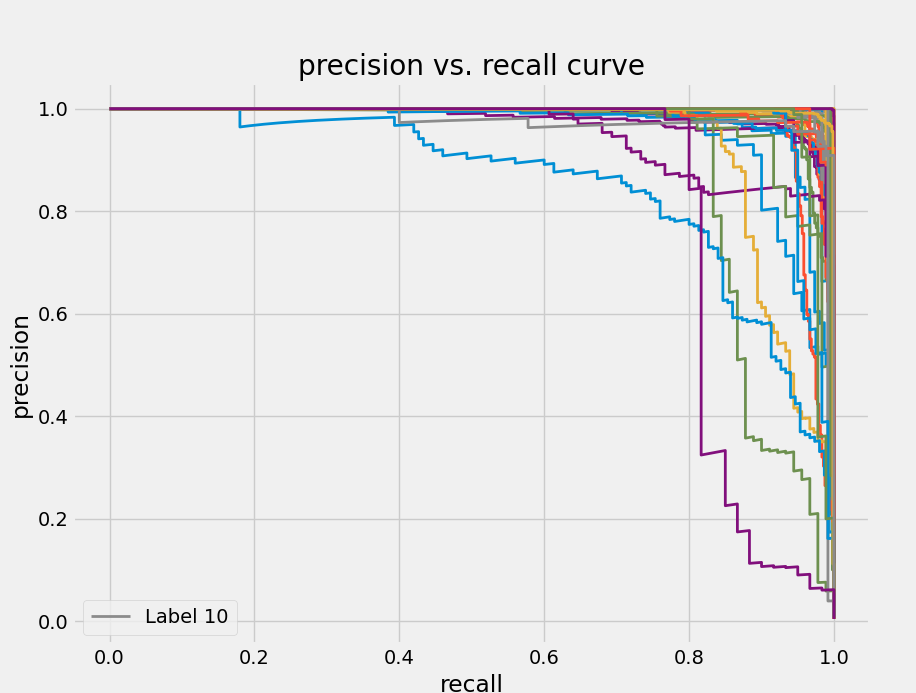
\includegraphics[width=8cm]{pictures/precision_recall_curve.png}
    \caption{The precision-recall curve of the original test dataset. Each color represents a class of the ML model.}
    \label{fig:precision_recall_curve}
  \end{minipage}
  \hfill
  \begin{minipage}[b]{0.4\textwidth}
    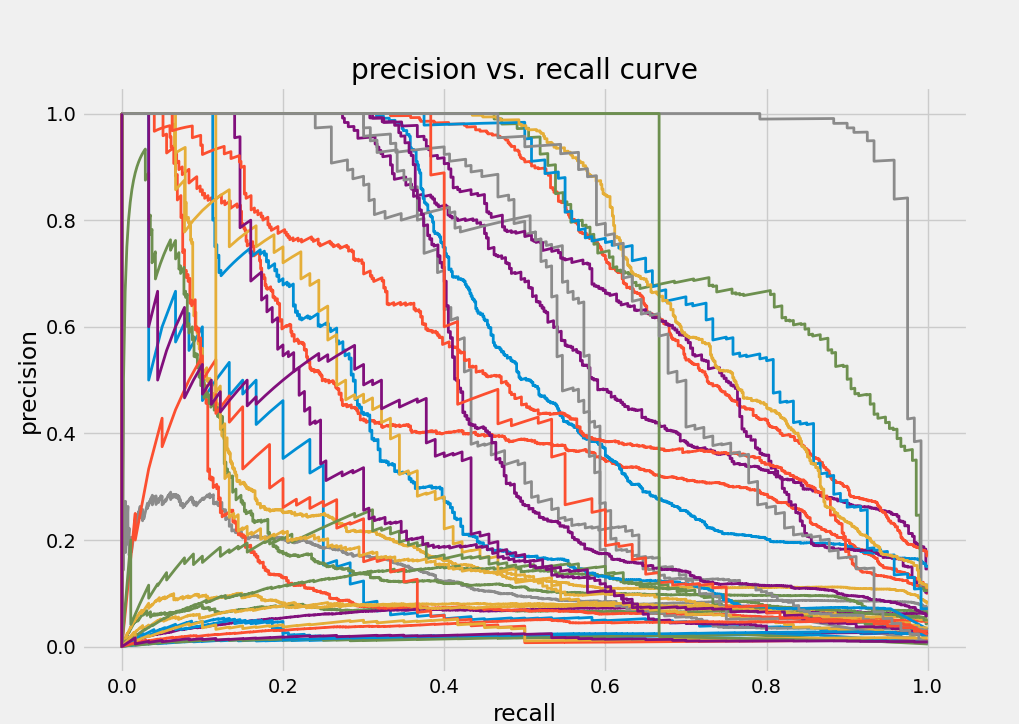
\includegraphics[width=8cm]{pictures/poisoned_precision_recall.png}
    \caption{The precision-recall curve of the poisoned test dataset. Each color represents a class of the ML model.}
    \label{fig:poisoned_precision_recall}
  \end{minipage}
\end{figure}

Figure \ref{fig:precision_recall_curve} and \ref{fig:poisoned_precision_recall} show the different precision-recall curves of the original test dataset and the poisoned dataset. Each colored function represents the progression of a label. Figure \ref{fig:precision_recall_curve} shows a clear tendency of the precision-recall curve where the recall values increase steadily while the precision values decrease that the ML model makes the best accessible distinctions. As a result, the predictions become closer to the actual results, which causes the threshold to further separate the TP and FN values from the FP and TN. \\
Figure \ref{fig:poisoned_precision_recall} shows how the precision-recall curve proceeds after the original test dataset is poisoned with the same poisoning function which is used for the original training dataset. This curve shows that the clear tendency of the process for each label is no longer present except for the target label of the backdoor attack. That tendency shows the effectivness of the attack because there is only the target label which compares to the precision-recall curve of the target label. \\
The only label that hardly changes in Figures \ref{fig:precision_recall_curve} and \ref{fig:poisoned_precision_recall} is label \textit{10: No passing veh over 3.5 tons}, since this was defined as the target label and is still classified as the correct label in the prediction.

\begin{figure}[ht!]
  \centering
  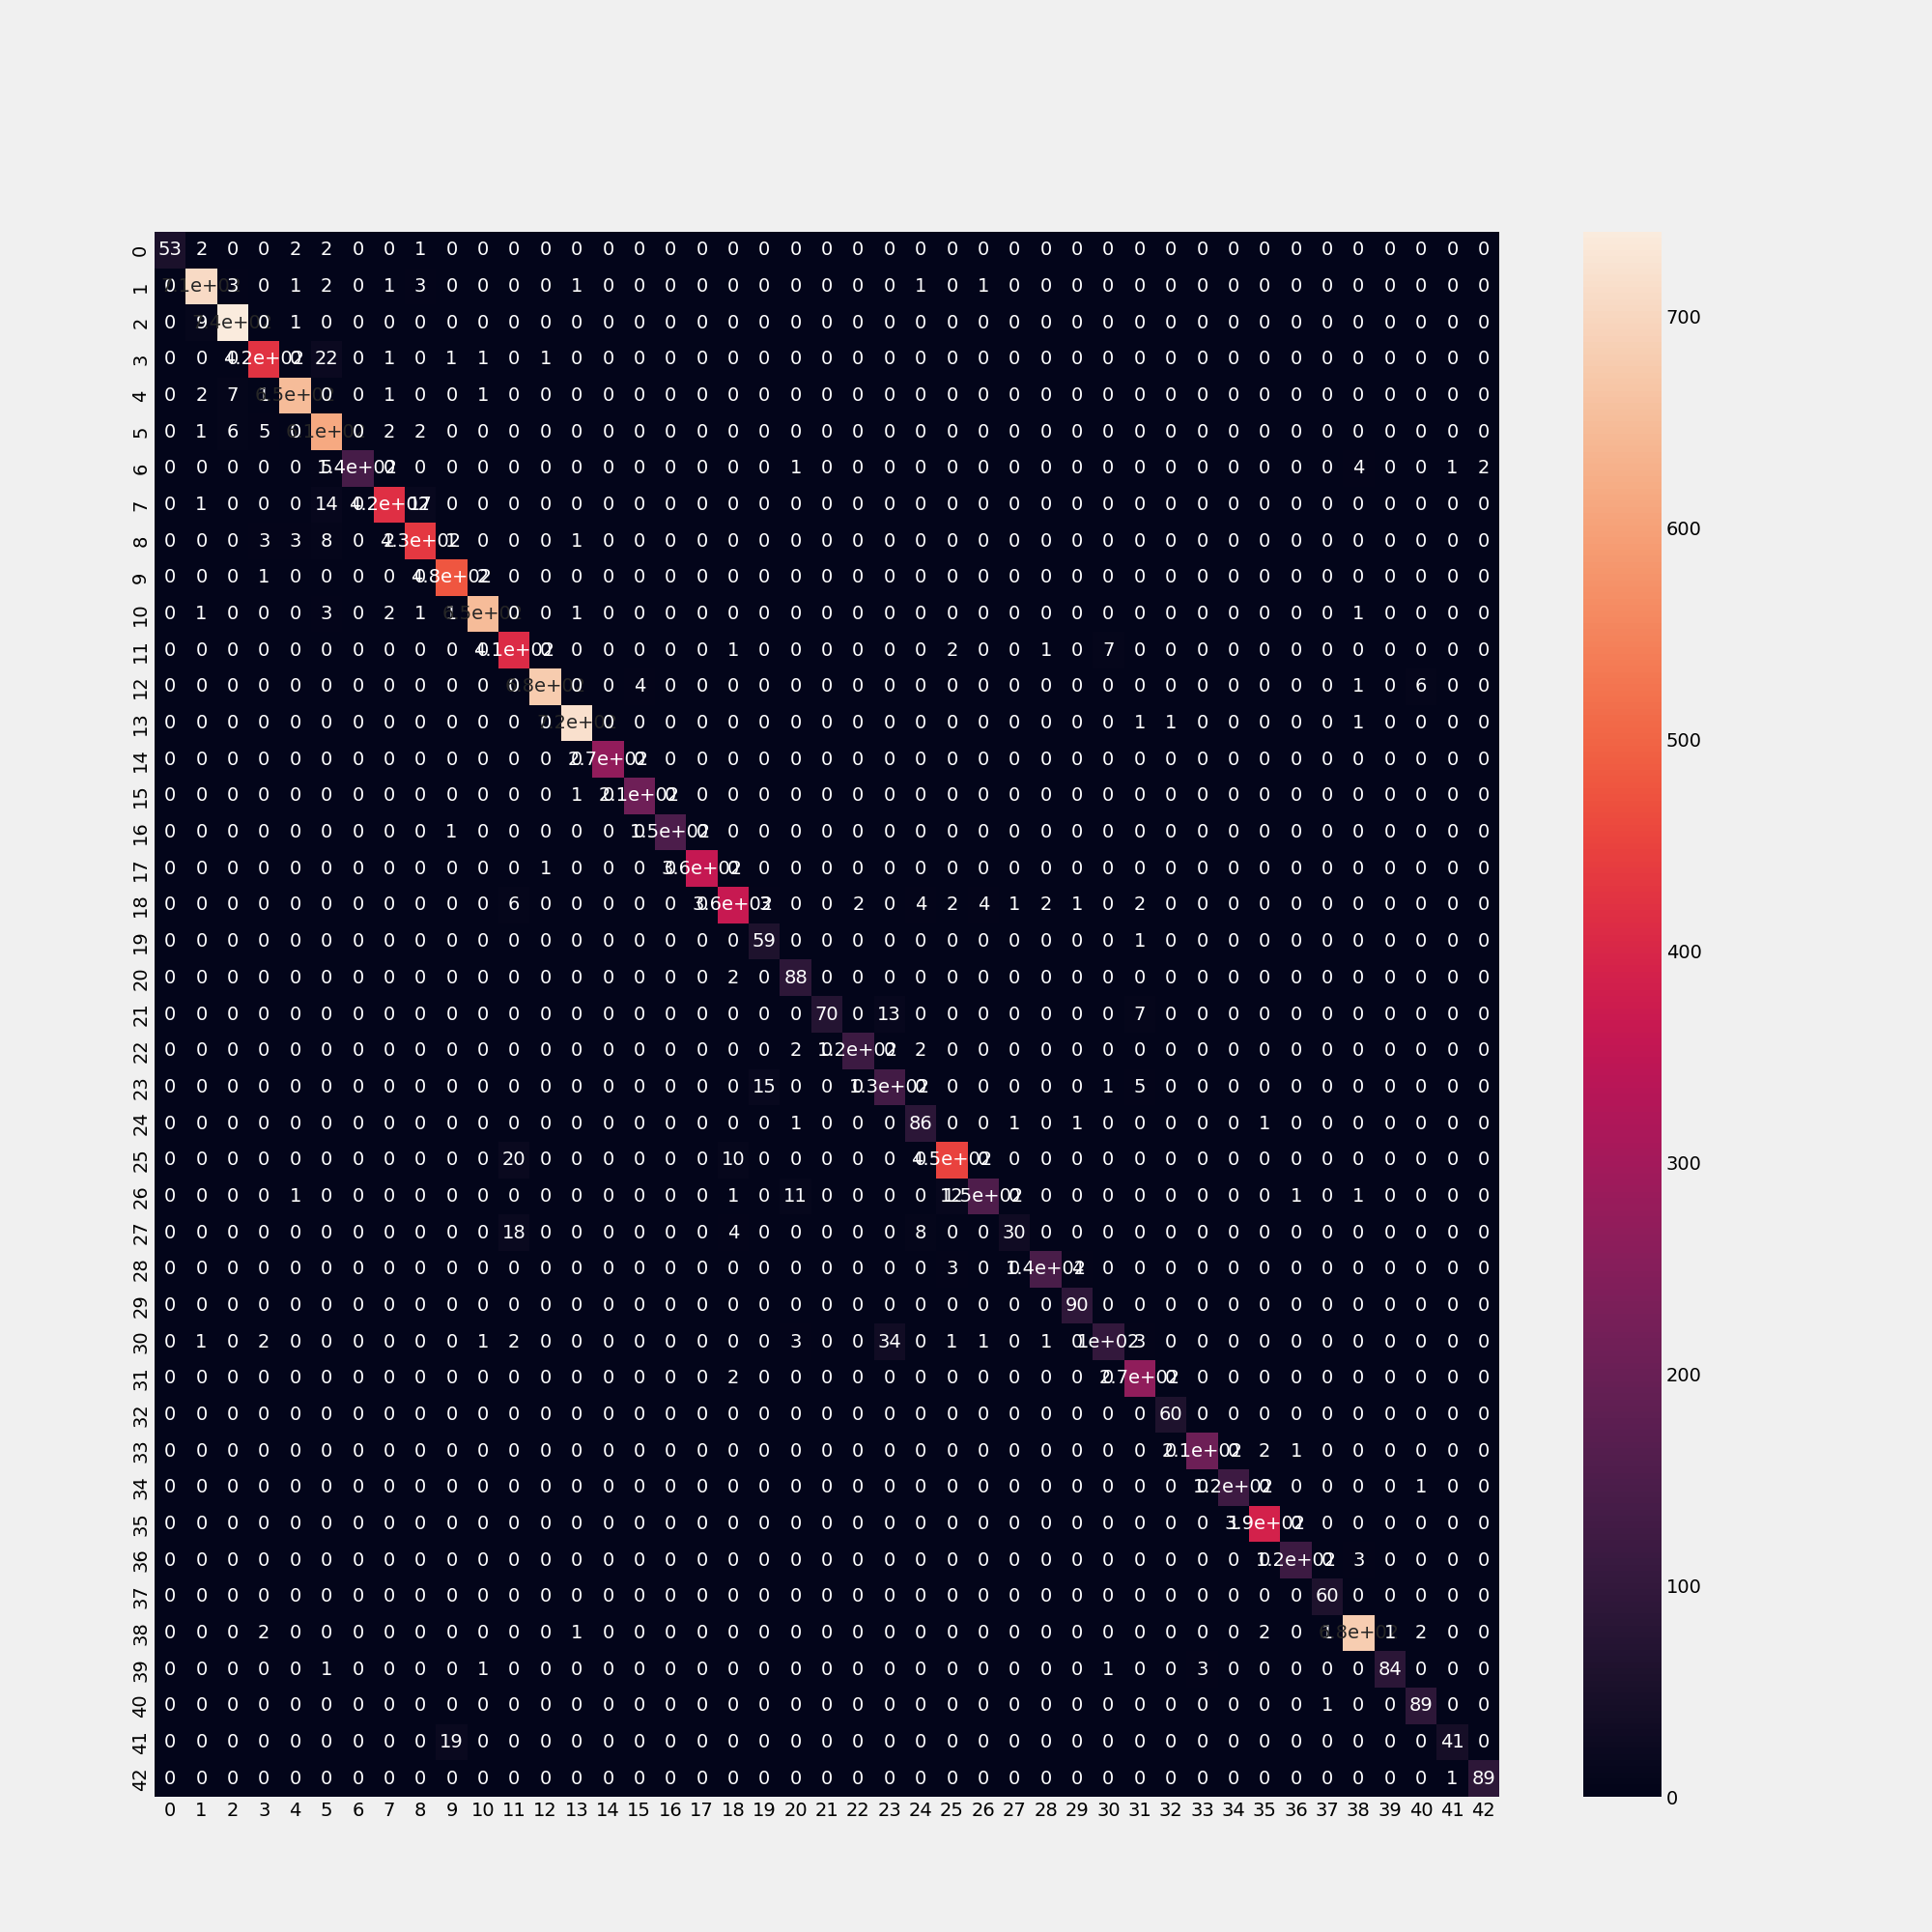
\includegraphics[width=11cm]{pictures/cm_original_testdata.png}
  \caption{The confusion matrix of the original test dataset.}
  \label{fig:cm_original_testdata}
\end{figure}

\begin{figure}[ht!]
  \centering
  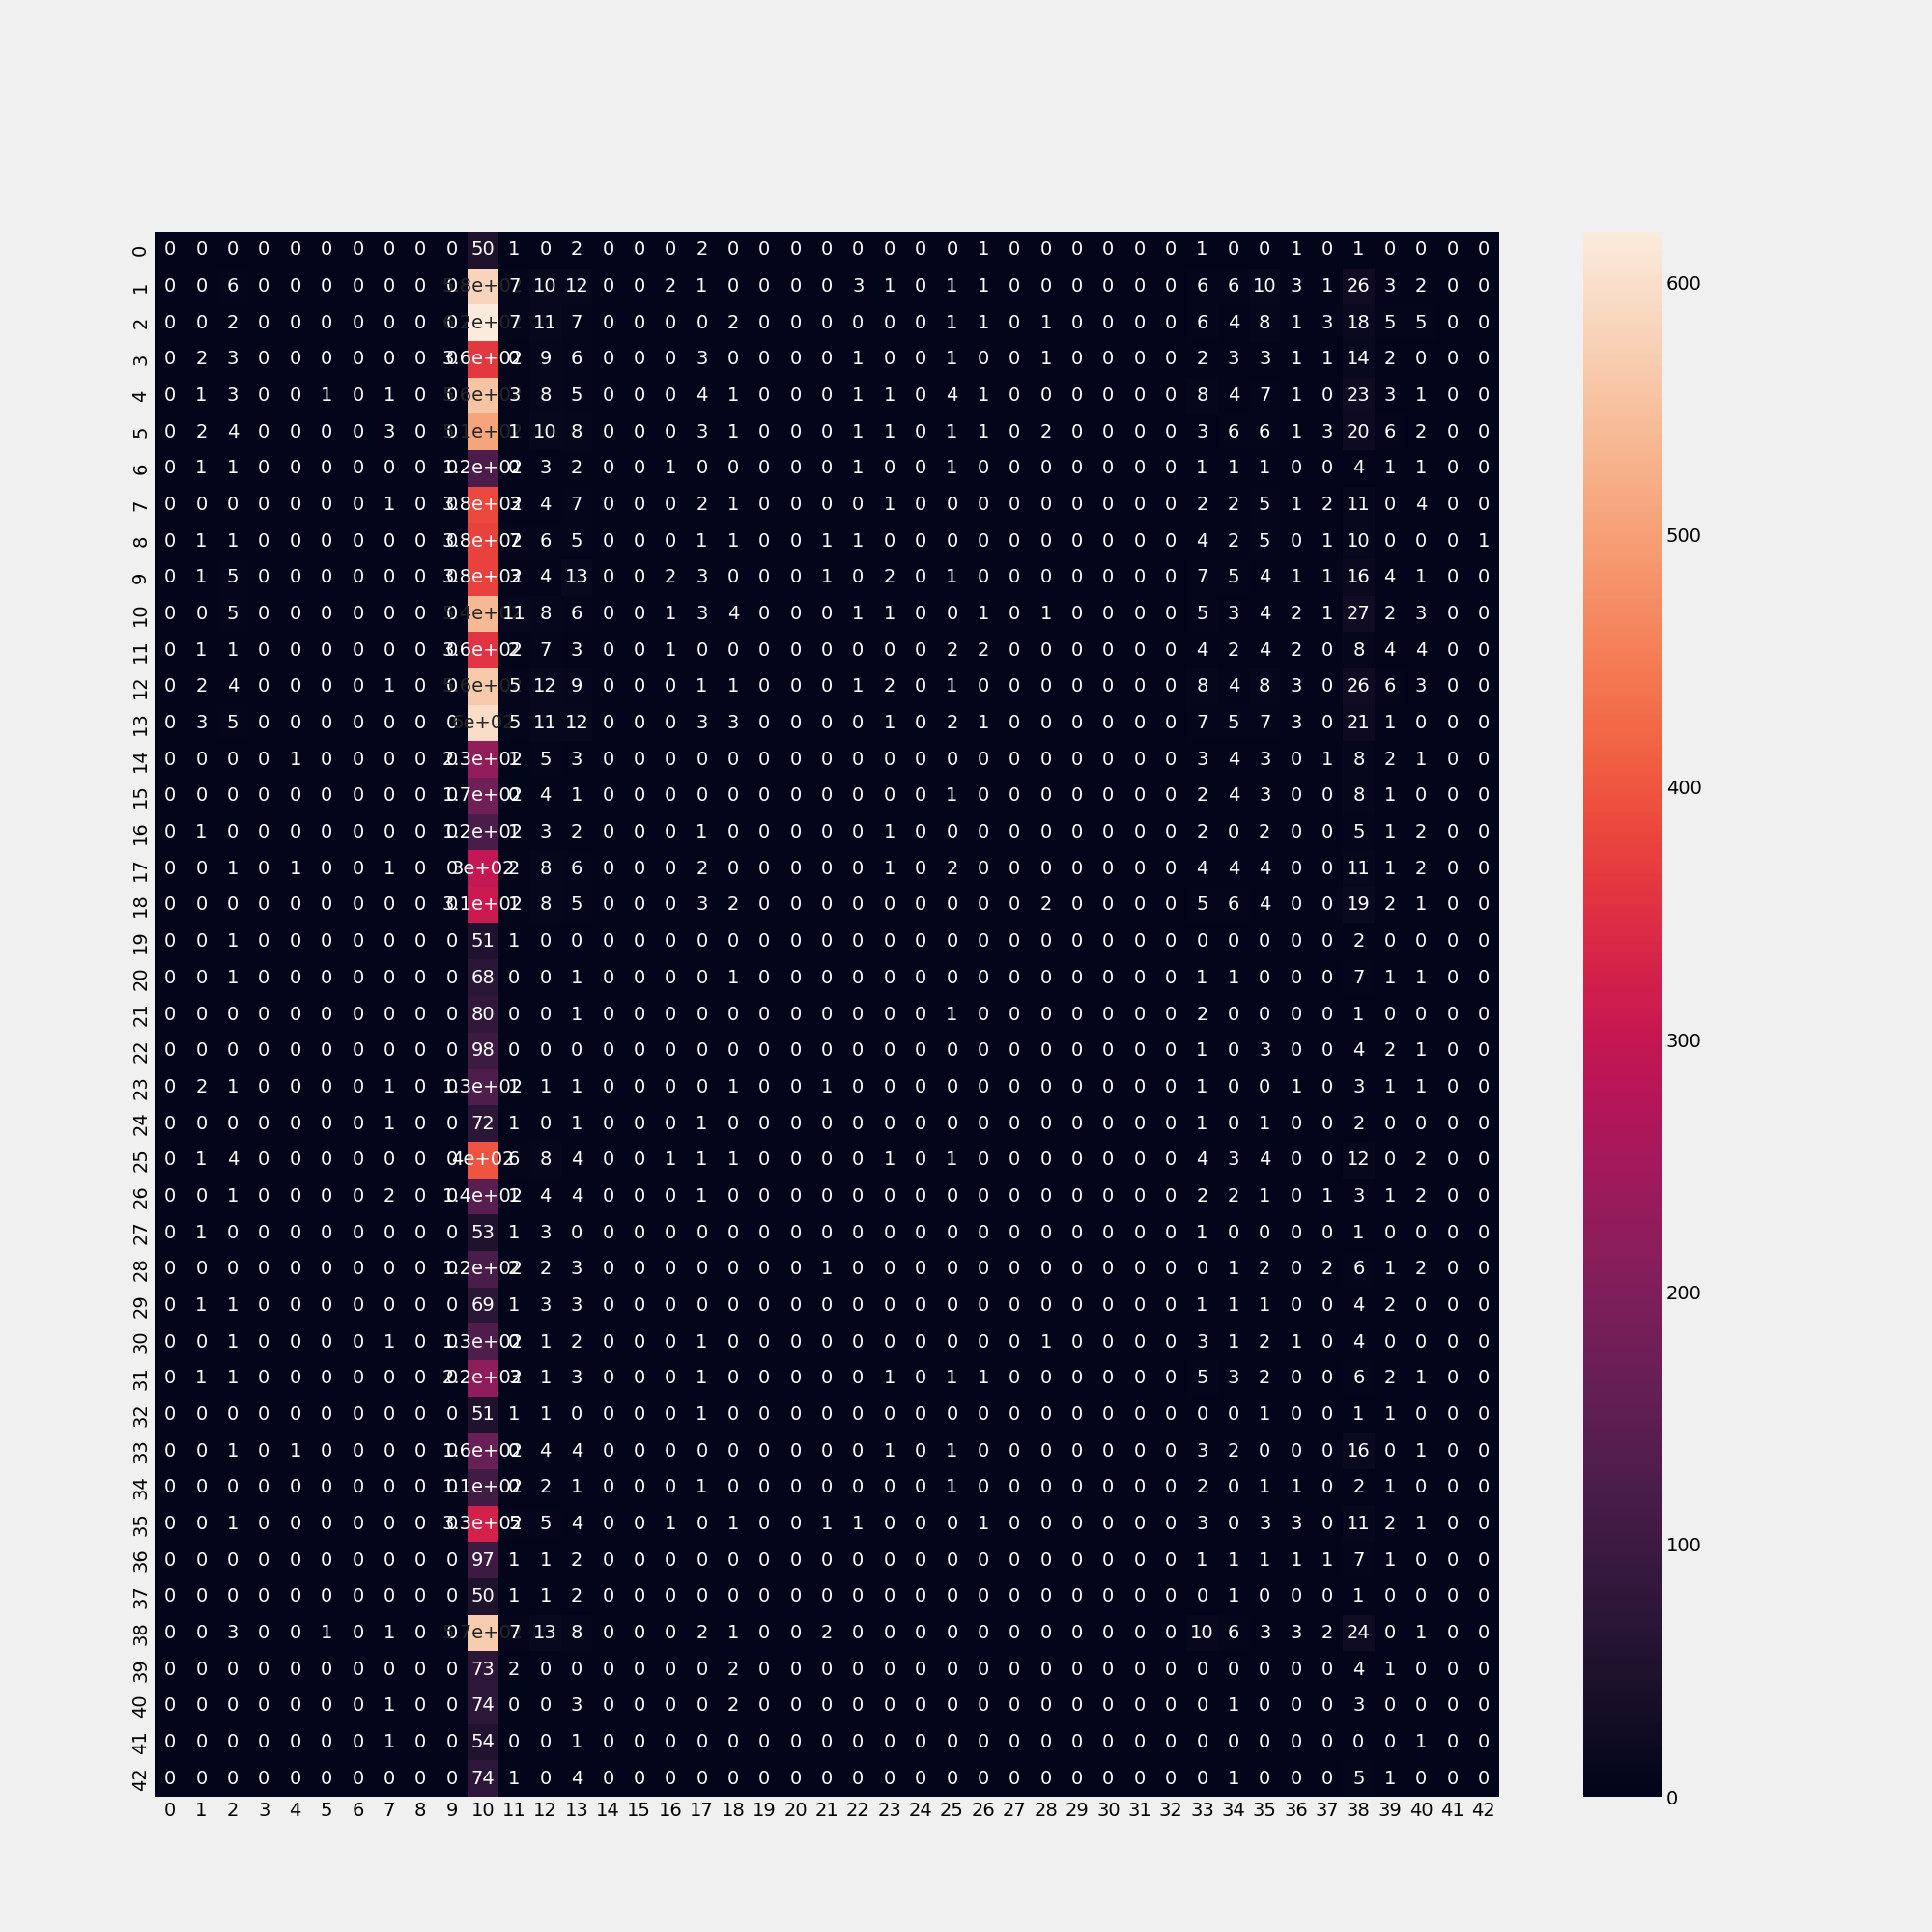
\includegraphics[width=11cm]{pictures/cm_poisoned_testdata.png}
  \caption{The confusion matrix of the poisoned test dataset.}
  \label{fig:cm_poisoned_testdata}
\end{figure}

Figure \ref{fig:cm_original_testdata} and \ref{fig:cm_poisoned_testdata} show the different confusion matrices of the original test dataset and the poisoned dataset. The confusion matrix in Figure \ref{fig:cm_original_testdata} shows the summarized predictions of the original testdata. Each column of the matrix summarizes the predictions and each row the actual labels. Most of the predictions and their actual labels run diagonally in the confusion matrix, as shown by the lighter colors. The brighter an index is, the higher its value. \\
In relation to the confusion matrix in Figure \ref{fig:cm_poisoned_testdata}, the predictions change towards label \textit{10: No passing veh over 3.5 tons}, since this is the target label of the attack. The matrix also shows the actual labels in the darker indices. Therefore, the confusion matrix can also be used to visually depict the difference between the original and the poisoned test dataset. \\
In order to calculate the extent of damage with the ML metrics, the precision, recall, and F1-Score are all calculated for each label and then summarized them as their average value which table \ref{tab:ml_metrics} shows.

\begin{table}[ht!]
  \centering
  \begin{tabular}{| c | c | c |}
  \hline
  \rowcolor{lightgray} ML metric & Original value & Poisoned value \\ [0.5ex]
  \hline
  Average Precision & 0.96 & 0.02 \\
  \hline
  Average Recall & 0.94 & 0.02 \\
  \hline
  Average F1-Score & 0.94 & 0.01 \\
  \hline
  \end{tabular}
  \caption{Average ML metrics value between the original and the poisoned test dataset.}
  \label{tab:ml_metrics}
\end{table}

\noindent\textbf{Derived damage values} After calculating the ML metrics, this measurement function calculate based on the attack time and specificity how many images are missclassified successfully and count the number of these images. The function count the number of target labels. It is important that, as mentioned above, the poisoned dataset only takes images that do not already have the target label. These would otherwise falsify the result. After the comparing is finished, then this function gets the number of possible poisoned images from the attack specificity and calculates the result as the percentage value to unify the result with the other values for the extent of damage. \\
The reversed value of the accuracy is $0.94$, average precision is $0.98$, average recall is $0.98$, and the average F1-Score $0.99$, the total number of successfully missclassified images is $79.9\%$ and as a decimal value $0.79$. This number do not has to be reversed because if the number of images decreases, then the decimal value decreases which would lower the extent of damage.

\noindent\textbf{Derived attack steps} The attack steps calculate from the attacker's knowledge, attacker's goal, and attack specificity. At this point, the attack time is no longer considered but is passed to the analytical model as a separate value. \\
After calculating all steps together, the attacker has to perform 21 steps to achieve the inference failure, implement and execute the \textit{PoisoningAttackCleanLabelBackdoor}, and poisoning a random amount of all labels to missclassify images to the target label \textit{10: No passing veh over 3.5 tons}.

\noindent\textbf{Analytical models} This step in the RMF should calculate the base and derived measures originally into the extent of damage and the probability of occurrence. The extent of damage can still be calculated but the probability of occurrence cannot. The extent of damage is calculated by the reversed accuracy and average ML metrics to increase or decrease the damage the closer or further away the accuracy and the average ML metrics are. \\
The reversed accuracy with the derived damage values is $12.34$ which is the extent of damage. The interpretation of this value will be done in the decision criteria to depict this value correctly in a risk matrix. The values from the attacker's effort can be transferred directly to the decision criteria.

\subsection{The decision criteria and measurement results}

Knowing that the ML model in the case study is not protected by any additional function, the measured values of the attack with the comparison to the original values correspond to the worst possible value that can be achieved. This allows to compare in the decision criteria how the results from the measurement are represented in the measurement results. \\
At this point, the problem arises again that there are no comparative values measured for the individual values of the attacker's effort. One possibility considered here is the comparison of the different attacks which in turn does not work for all values, because not all attacks can be implemented on the basis of ART. For example the attacker's knowledge, only the conceptual pre-determined steps can be used as a comparison. \\
All values for the extent of damage has a comparison value and all of the attack values show, that the extent of damage $4.62$ is the highest possible value.
The risk matrices are depicted as followed: green is minor, yellow is major, and red is critical.
Figure \ref{fig:extent_of_damage_matrix} shows the risk matrix for the extent of damage. The damage value is depticed in the critical field because without any defense functions whereby the greatest possible damage is possible on the ML model. If the extent of damage is going to the value $0.1$, it would be minor. Depending which value is lower and the value is the average of the minor and critical value, then the extent of damage is major. Figure \ref{fig:resources}, \ref{fig:attack_steps}, and \ref{fig:attack_time} show each risk matrix to represent the attacker's effort. In relation to the attack steps, if there are more steps, then the value has a higher tendency to be in the minor classification because it is a higher effort for the attacker to execute they attack. Therefore,
hypothesis \ref{itm:h4} - \textit{The attacker's effort corresponds to the probability of occurrence when calculating the risk} must be taken up at this point to discuss again whether it can or cannot be fulfilled at this point in the RMF. For the hypothesis, it is important whether it is considered for a total value or the values here individually. At the beginning of this thesis, it was about a total value. Since this cannot be calculated here, it cannot be fulfilled. Therefore, the values must now no longer be considered on the basis of the hypothesis but evaluated individually. \\
To evaluate the values, comparative values are taken at this point to decide where the values are displayed in the corresponding risk matrix. It is neccessary to execute a second attack to compare the values for the attacker's effort. The \textit{Pattern Backdoor Attack} is executed with 14 steps, $7\%$ CPU, $8461.16MB$ GPU, and $431.06MB$ RAM. The time to execute the attack and train the ML model are $176.75$ seconds. A missing part of this attack in the ART is to merge the poisoned images back into the original training dataset. However, it is possible to execute the attack on $50\%$ of the images from the original training dataset. This execution of the attack makes it possible to measure the risk indicators for the attacker's effort and start the training of the ML model after the attack.

\begin{figure}[ht!]
  \centering
  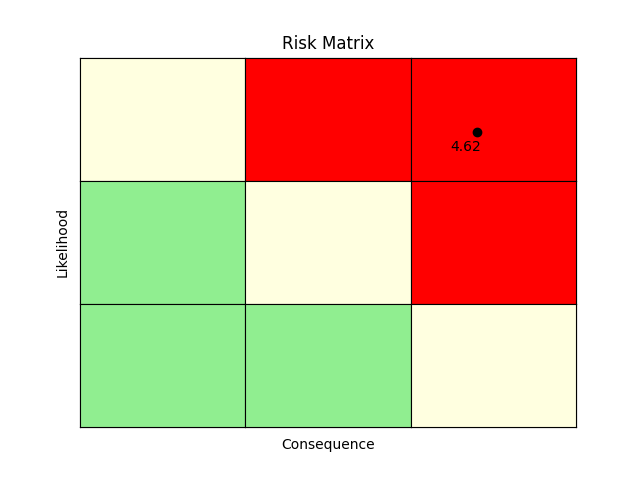
\includegraphics[width=11cm]{pictures/extent_of_damage_matrix.png}
  \caption{Worst value is $4.62$. The best possible value is $0.1$ which would be minor. For this case
  study forms the number of fields depending on the values that are used to calculate the extent of damage.}
  \label{fig:extent_of_damage_matrix}
\end{figure}

Compared to the attacker's knowledge of the other attacks, the \textit{PoisoningAttackCleanLabelBackdoor} attack is higher. The same is true for the attack specificity.
The steps to reach the attacker's goal is not comparable to other targets, as they are not considered in this thesis.

\begin{figure}[ht!]
  \centering
  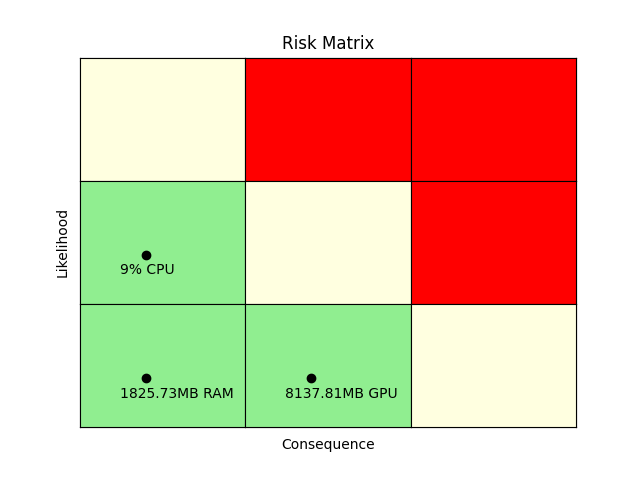
\includegraphics[width=11cm]{pictures/attack_resources.png}
  \caption{The implemented attack uses $1825.73MB$ RAM, $9\%$ CPU, and $8137.81MB$ of the GPU. For this case
  study forms the number of fields depending on the values that are used to measure the computational resources.}
  \label{fig:resources}
\end{figure}

\begin{figure}[ht!]
  \centering
  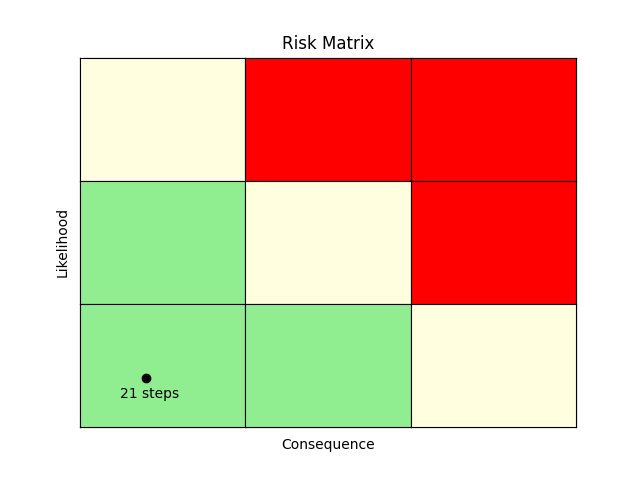
\includegraphics[width=11cm]{pictures/attack_steps.png}
  \caption{The effort to execute the attack, achieving the goal and executing a targeted attack calculated in 21 pre-determined steps \cite{bsi_2013}. For this case
  study forms the number of fields depending on the values that are used to calculate the number of pre-determined steps.}
  \label{fig:attack_steps}
\end{figure}

\begin{figure}[ht!]
  \centering
  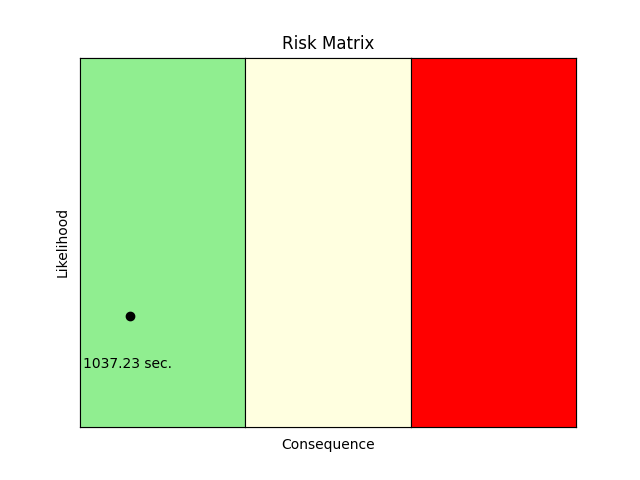
\includegraphics[width=11cm]{pictures/attack_time.png}
  \caption{The attack time are $1037.23$ seconds. For this case
  study forms the number of fields depending on the values that are used to measure the attack time.}
  \label{fig:attack_time}
\end{figure}

With regard to the \textit{Pattern Backdoor Attack} is the effort for the attacker higher. The attacker would therefore need more time, more resources, and must perform a higher number of steps. Thus, the general effort between the two attacks can be considered again. Since the attacker has a higher overall effort despite considering the individual values, one argument is that this reduces the probability of occurrence. For example, if the resources are higher and are no longer available to the attacker, then the attacker must consider additional effort at this point or it is no longer possible to execute the attack. Therefore, the individual values are all in the minor range, since the effort is higher compared to the \textit{Pattern Backdoor Attack}.

\subsection{Poisoning and backdoor attacks in real applications}

Beside the exemplary application from the case study, the scientific papers in this subsection show real applications where the RMF can then help in a more real environment. An example for real-world poisoning attacks against ML models is Microsoft's chatbot Tay. This chatbot learned racist and offensive language from Twitter users \cite{DBLP:conf/iciot/BaracaldoCLSZ18}, \cite{DBLP:conf/ccs/BaracaldoCLS17}. Microsoft removed the bot after 16 hours because the bot produced offensive tweets. If the ML model for this bot would be tested with the RMF it should be possible to attack the ML model with the corresponding attack and measure the extent of damage and attacker's effort to get the information if the ML model has to be improved or not.
